\articlehead{Convention Mystique}{Makyo}{2011}

I was too excited to sleep, the night before Anthrocon 2005.  It was the first convention I would be going to, I'd be meeting some truly awesome people for the first time basically the minute I stepped into the hotel, and sleep just wasn't going to happen.  In order to make sure that I could make it down to the airport without crashing or anything, I planned on subsisting almost completely on black tea through the night, then stopping on Starbucks twice on the way down from Fort Collins to Denver.  Unfortunately, both my roommates were asleep, so I was listening to music on my headphones.  I had forgotten that I had put the kettle on for tea, so I was interrupted from my jittery reverie by my roommate knocking on my door to inform me that the kettle had been whistling for five minutes or so by that point.  I was lucky I hadn't boiled it dry.

With the lack of sleep and my excitement, I was basically useless for the first day of the convention.  I got into Philadelphia at around 2:30 or so in the afternoon and to the hotel by 3PM.  I stumbled into the lobby and met, for the first time, my friends, some of whom I had known for five years, by that point.

Due to my age and some lingering doubts about meeting furries, I had never really planned on going to a convention, at least not until the beginning of 2005.  I had met furries in person before, of course; my partner and I had visited each other on several occasions for the years previous, and I had a small group of furry friends around me throughout high school and moving into college.  It wasn't really until March or April of 2005 that I started really meeting more and more members of the fandom, and then only when I was dragged to a local furmeet by a friend of mine, where I had plenty of fun.

The problem with conventions for me until that point was two-fold: first of all, there was this negative stereotype floating around about who furries were and how they interacted with each other -- the most succinct comment to this was the oft-quoted ``by and large, furries are bi and large'' -- which I found vaguely disturbing; and secondly, I was so used to interacting with my friends online that I wasn't quite sure how well interacting in person with them was going to work out.  I knew, for instance, that my friend was a five and a half foot tall red fox on the Internet, but I had been assured that he was a good bit taller and most likely not actually a fox in person.  How would I interact with him?  I knew for sure that I wasn't also a fox, so there were probably certain things that we were used to doing that wouldn't likely happen in person: no swishing, for instance, and there would probably a dearth of nuzzling, murring, and all the rest.

Having started to interact more with furs offline, however, much of my fears were allayed, and I warmed quickly to the concept of heading out to a convention.  The people I had been meeting were normal people, and we had a ready-made topic of conversation.  I figured things would be fine with a few more of them around.  I pulled my money together and flew out to the final Anthrocon in Philly.  Rather than finding a bunch of normal people milling around with a ready-made topic of conversation, though, I found that conventions were a little more complicated than just that.

For me, the first con was all about validation.  It wasn't so much that I was around a bunch of people who could talk about the latest fursuit they'd seen or bit of gossip they heard.  It was more than just a group of people, period.  Furry wasn't something we did, it was something we were.  I hadn't understood the concept of a furry lifestyle until then, but that certainly cemented home the fact that we weren't just partaking in a hobby, but interacting with others who also had this integral part of their lives, and expressing that with them.  I don't really mean to wax rhapsodic about my first con, it wasn't all sunshine and scritches, just that it was certainly more than I had hoped for: my friends and I got along just as wonderfully in person as we did online.

It also helped drive home the idea that conventions are more than just a bunch of people interacting in person rather than online.  I talked to several of my friends that I had met at the local furmeet online and interacting in either location was just a matter of either typing or talking, it didn't matter which.  A convention, however, is more a unique medium.  It's not just a big furmeet, and it's not just furries interacting offline instead of on; everything works slightly differently in a con setting.  It's as if, after a certain number of attendees (lets say twenty five), or in a certain location (almost always a hotel), we cease being interested parties and become a little society of our own, with our own mores and modes of interaction.

\begin{wrapfigure}{l}{0.3\textwidth}
  \begin{center}
    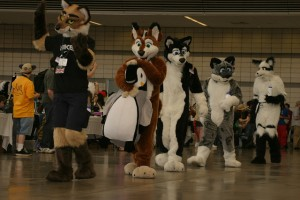
\includegraphics[width=0.25\textwidth]{content/assets/convention-mystique--parade}
  \end{center}
\end{wrapfigure}
Since I was pretty effectively hooked after that first convention, I did my best to head to several more after that, making several more Anthrocons and man Further Confusions, as well.  While I enjoyed my first few conventions in a near ecstatic state, I settled down soon after to relax and enjoy my time in these new surroundings and  in this new society.  Conventions have a rhythm to them, a tempo, or a curve.  There's the building excitement leading up to the trip, the hassle of packing and flying, and the first exciting few hours catching up with your friends and having a few drinks, then the sustained joy over the next few days until things start to wind down, with more people leaving the area, having to go to bed early to make their early flights, crying in the hallways, lobby, and airport.  It's something you settle into like a comfortable sort of routine.  Every convention's different, of course, but I think the general experience follows that same ramp up, sustained level, then tapering off, even if, in the case of Camp Feral, there's that last trip back out of the woods tossed in.

There are a few other seeming universals tossed in along with the convention.  It does seem possible to break the attendees down into several fairly constant categories:

\begin{description}
  \item[The New Attendee] Bright eyed, in the throes of ecstasy, the new attendee is easy to pick out from all other groups (excepting perhaps The Nut) as the one who is mostly gung-ho about everything.  They want to go to all the events, the want to ogle all the suits, they want to hug all their friends.  These folks are really relatively harmless, and they help keep the conventions exciting for those who frequent them.
  \item[The Nut] Similar to The New Attendee, this person is totally gung-ho about everything, except that it's almost certainly not their first con.  They have the relentless, determined enthusiasm that drives many groups to go to events or check out new restaurants in the area, or, on the flipside, drives many people nuts.  While it's nice to keep some of that joy from the first visit to a furry con, and it certainly is good to keep experiencing them, sometimes it's best to just calm down, breathe\ldots
  \item[The Lobby Lounger] Sitting in the lobby and ordering a ceaseless round of drinks (even if they're just waters), drawing and kibitzing, texting all their friends to tell them to “just meet me in the lobby”, this attendee is a near permanent fixture in the lobby of the main hotel, preferring to soak the con up rather than necessarily go out and experience it in panels and the like.
  \item[The Wanderer] Wandering from lobby to Dealer's Den to Artist's Alley to the panels to their room to restaurants to the lobby ad nauseum, this person is easy to find, but not so easy to pin down for plans -- why stop? They might miss something!  Of course, having spent the whole convention wandering around, there's a chance they actually saw less than the might have otherwise.  An important sub-category of this is The Fursuiter, who wanders around with good reason -- it's hard to do anything in one place for long without overheating or, heaven forbid, not get quite enough attention.
  \item[The Worker] There's always money to be made at conventions, or if not money, a little bit of power, however benign.  The Worker is the artist who will work their way through the con to hopefully come out of the affair net positive, or the volunteer who will check badges at the door to do their part for the convention.  Even if it might be difficult to to see them for more than a few minutes at a time, they're still an integral part of the con atmosphere.
\end{description}


\begin{wrapfigure}{r}{0.3\textwidth}
  \begin{center}
    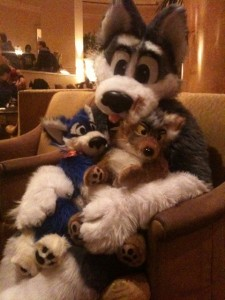
\includegraphics[width=0.25\textwidth]{content/assets/convention-mystique--plush}
  \end{center}
\end{wrapfigure}
There's another universal almost too obvious to mention: convention badges.  Most any convention has their own, obviously, but within our fandom, it's customary to not only wear the membership badge, but also art badges created specifically for the wearer.  These small, commissioned bits of wearable art represent the owner's character, another unique artifact of the difference between our selves and our characters.  So unique, in fact, that, concurrent with the upcoming Further Confusion, there will be a portion of a gallery exhibition in San Jose dedicated strictly to the art of the con badge.  They act as a way to help carry our characters into our real-life interactions and blur the line between the two somewhat.  We may not all be dressed up like our creations, nor can we all swish and bark and so on, but at least we have a sign of just who we are visible to those around us.

Of course, anyone who has been to a furry convention knows the basic duck-and-weave of the con greeting.  With the near-absolute saturation of con badges, it's be come standard practice to approach someone looking at their chest, sleeves, or belt, wherever they've hung their badges.  Depending on how friendly you are and whether or not you know the other person, you might jump straight into a hug after that, or start chattering right away.  If you don't know them, of course, you still know more about them after that brief glance than you might if you had just met on the street, and that's something we've written about before.  It gives a whole new meaning to “my face is up here” (and, of course, if you put a QR code on your badge, now they're pointing a camera at their chest\ldots).

The mystique surrounding the convention and the medium of interaction that it represents is an integral part of the fandom.  For many, our conventions are the high point of the year, a time to both see friends we rarely get the chance to see and blur the line between our selves and our characters.  It's the time when we get to let down our guard somewhat and show some of our back-stage selves, show some emotion with how we feel about our little subculture, and maybe even act a fool in a giant animal costume.  They're the time for us to live out our culture in person.  It's interesting that, with a group based so strongly on interaction on the Internet, some of our highest points are the times when we get off the ‘net and hang out in person -- whether it be to relax, to have fun, or to make money.

I'll see you guys at Further Confusion 2012!
